Los sistemas robóticos y de realidad virtual y aumentada (VR/AR) modernos abarcan un espectro amplio de plataformas: desde nano drones y robots móviles de bajo costo, con CPU embebidas, sin GPU dedicada y baterías de capacidad reducida, hasta headsets de VR/AR de alta gama y robots equipados con hardware especializado (Figura~\ref{fig:devices}). A pesar de esta diversidad, todos comparten una misma presión de diseño: la eficiencia del sistema de percepción importa de manera fundamental, independientemente de los recursos disponibles. Para las plataformas más restringidas, la eficiencia es directamente una condición de viabilidad. Pero incluso en plataformas con mayor capacidad computacional, un sistema de percepción liviano se traduce en mayor autonomía de batería, menor carga térmica, y mayor disponibilidad del hardware dedicado para otras tareas críticas, como el renderizado en tiempo real en aplicaciones de VR/AR, o la planificación de movimiento en robótica de alta velocidad. Diseñar sistemas de percepción eficientes es una propiedad deseable en cualquier plataforma.

Para que un robot o dispositivo de VR/AR opere de manera útil en el mundo real, necesita saber dónde se encuentra en el espacio. Esta capacidad, conocida como localización, es fundamental: sin ella, un drone no puede navegar, un robot no puede planificar trayectorias, y un headset de realidad aumentada no puede anclar objetos virtuales al entorno físico de manera coherente. La manera más directa de estimar la pose es mediante la odometría: integrar las mediciones de los sensores para recuperar la trayectoria recorrida de forma incremental. Sin embargo, la odometría pura acumula error con el tiempo, sin mecanismo alguno para corregirse. El SLAM (Simultaneous Localization and Mapping) \cite{cadena2016slam} extiende este enfoque construyendo además un mapa persistente del entorno, lo que habilita dos capacidades esenciales para la operación prolongada: la detección y cierre de ciclos (loop closure) \cite{tsintotas2022revisiting}, que permite reconocer lugares ya visitados y corregir el error acumulado en la trayectoria, y la reutilización del mapa, que permite relocalizarse en entornos conocidos sin reconstruirlos desde cero.

Las cámaras son sensores atractivos para la odometría: son baratas, ligeras, y capturan información rica del entorno. Sin embargo, estimar el movimiento a partir de imágenes (odometría visual) es inherentemente frágil ante movimientos rápidos, escenas poco texturadas o iluminación deficiente. Las unidades de medición inercial (IMUs), por su parte, miden aceleraciones y velocidades angulares a alta frecuencia y son robustas ante estas condiciones, pero integrar sus mediciones acumula error (drift) de manera cuadrática. La fusión de ambos sensores da origen a la odometría visual-inercial (VIO), que combina la riqueza de la información visual con la alta frecuencia y robustez de la IMU, obteniendo estimaciones de pose precisas incluso en condiciones desafiantes. Al incorporar la construcción de un mapa persistente sobre VIO se obtiene el VI-SLAM (Visual-Inertial SLAM), que integra las fortalezas de ambos sensores con las capacidades de corrección a largo plazo propias del SLAM.
% TODO: introducir partes de un sistema de slam: front-end, detection, tracking, optimization, place recognition?

A pesar de los avances significativos en las tecnologías VIO \cite{leutenegger2015okvis, usenko2020basalt} y VI-SLAM \cite{campos2021orbslam3, leutenegger2022okvis2, ruckert2021snakeslam} de los últimos años, los sistemas actuales enfrentan dificultades para satisfacer simultáneamente los tres requisitos que exige el despliegue en plataformas reales: precisión en la estimación de pose, eficiencia computacional para operar en tiempo real con bajo consumo de recursos del sistema, y robustez ante las condiciones adversas típicas del mundo real, como escenas de baja textura, movimientos bruscos o trayectorias de larga duración. Los métodos puramente geométricos, que no dependen de redes neuronales o hardware especializado, constituyen la alternativa más eficiente y portable para el despliegue en sistemas reales, pero incluso los sistemas del estado del arte presentan dificultades para garantizar robustez y procesamiento en tiempo real en condiciones realistas~\cite{demayo2025monadoslamdataset}.

Este trabajo presenta un sistema de VI-SLAM diseñado para abordar estas limitaciones. El sistema está basado en Basalt~\cite{usenko2020basalt}, un sistema VIO del estado del arte orientado originalmente a aplicaciones de VR/AR, y extiende el trabajo previo~\cite{zanotti2024basaltxr} extendiendo la gestión del mapa persistente con múltiples operaciones. El mapa es gestionado de manera inteligente mediante una arquitectura de comunicación asíncrona entre componentes, lo que permite que las operaciones costosas asociadas al mantenimiento del mapa, como la detección de ciclos, la optimización global y el culling de keyframes, se ejecuten sin degradar el rendimiento del sistema principal. La detección de ciclos se realiza mediante HashBoW~\cite{hashbow2024stricker}, un método eficiente de recuperación de keyframes por similitud visual. La corrección del error acumulado se efectúa mediante Pose Graph Optimization (PGO), y la consistencia del mapa a largo plazo se garantiza mediante fusión de mapa y heurísticas de eliminación de keyframes que priorizan aquellos de alta calidad visual y espacial. Adicionalmente, se propone un método de bundle adjustment eficiente y numéricamente estable, basado en RootBA~\cite{demmel2021largescalerootba}, que adapta la formulación mediante factorización QR al caso de sistemas multicámara con modelos de cámara arbitrarios y soporta ejecución en precisión simple, con beneficios sustanciales de rendimiento.

El desempeño del sistema propuesto se evalúa de manera exhaustiva sobre datasets públicos del estado del arte como EuRoC~\cite{burri2016euroc}, TUM-VI~\cite{schubert2018tum} y el Monado SLAM Dataset~\cite{demayo2025monadoslamdataset}, que cubren una amplia variedad de escenarios representativos de robótica y VR/AR, incluyendo entornos con baja textura, movimientos rápidos y trayectorias de larga duración. La evaluación mide precisión y rendimiento computacional, comparando el sistema contra dos alternativas del estado del arte. Los resultados muestran que el sistema alcanza una precisión comparable al estado del arte, particularmente en entornos típicos de VR/AR; mantiene la operación en tiempo real incluso en trayectorias de larga duración; y exhibe robustez ante condiciones adversas. El método de bundle adjustment propuesto resulta numéricamente estable y su ejecución en precisión simple produce una mejora de rendimiento considerable respecto a la precisión doble.

\begin{figure}[ht]
    \centering
    \begin{subfigure}[b]{0.30\textwidth}
        \centering
        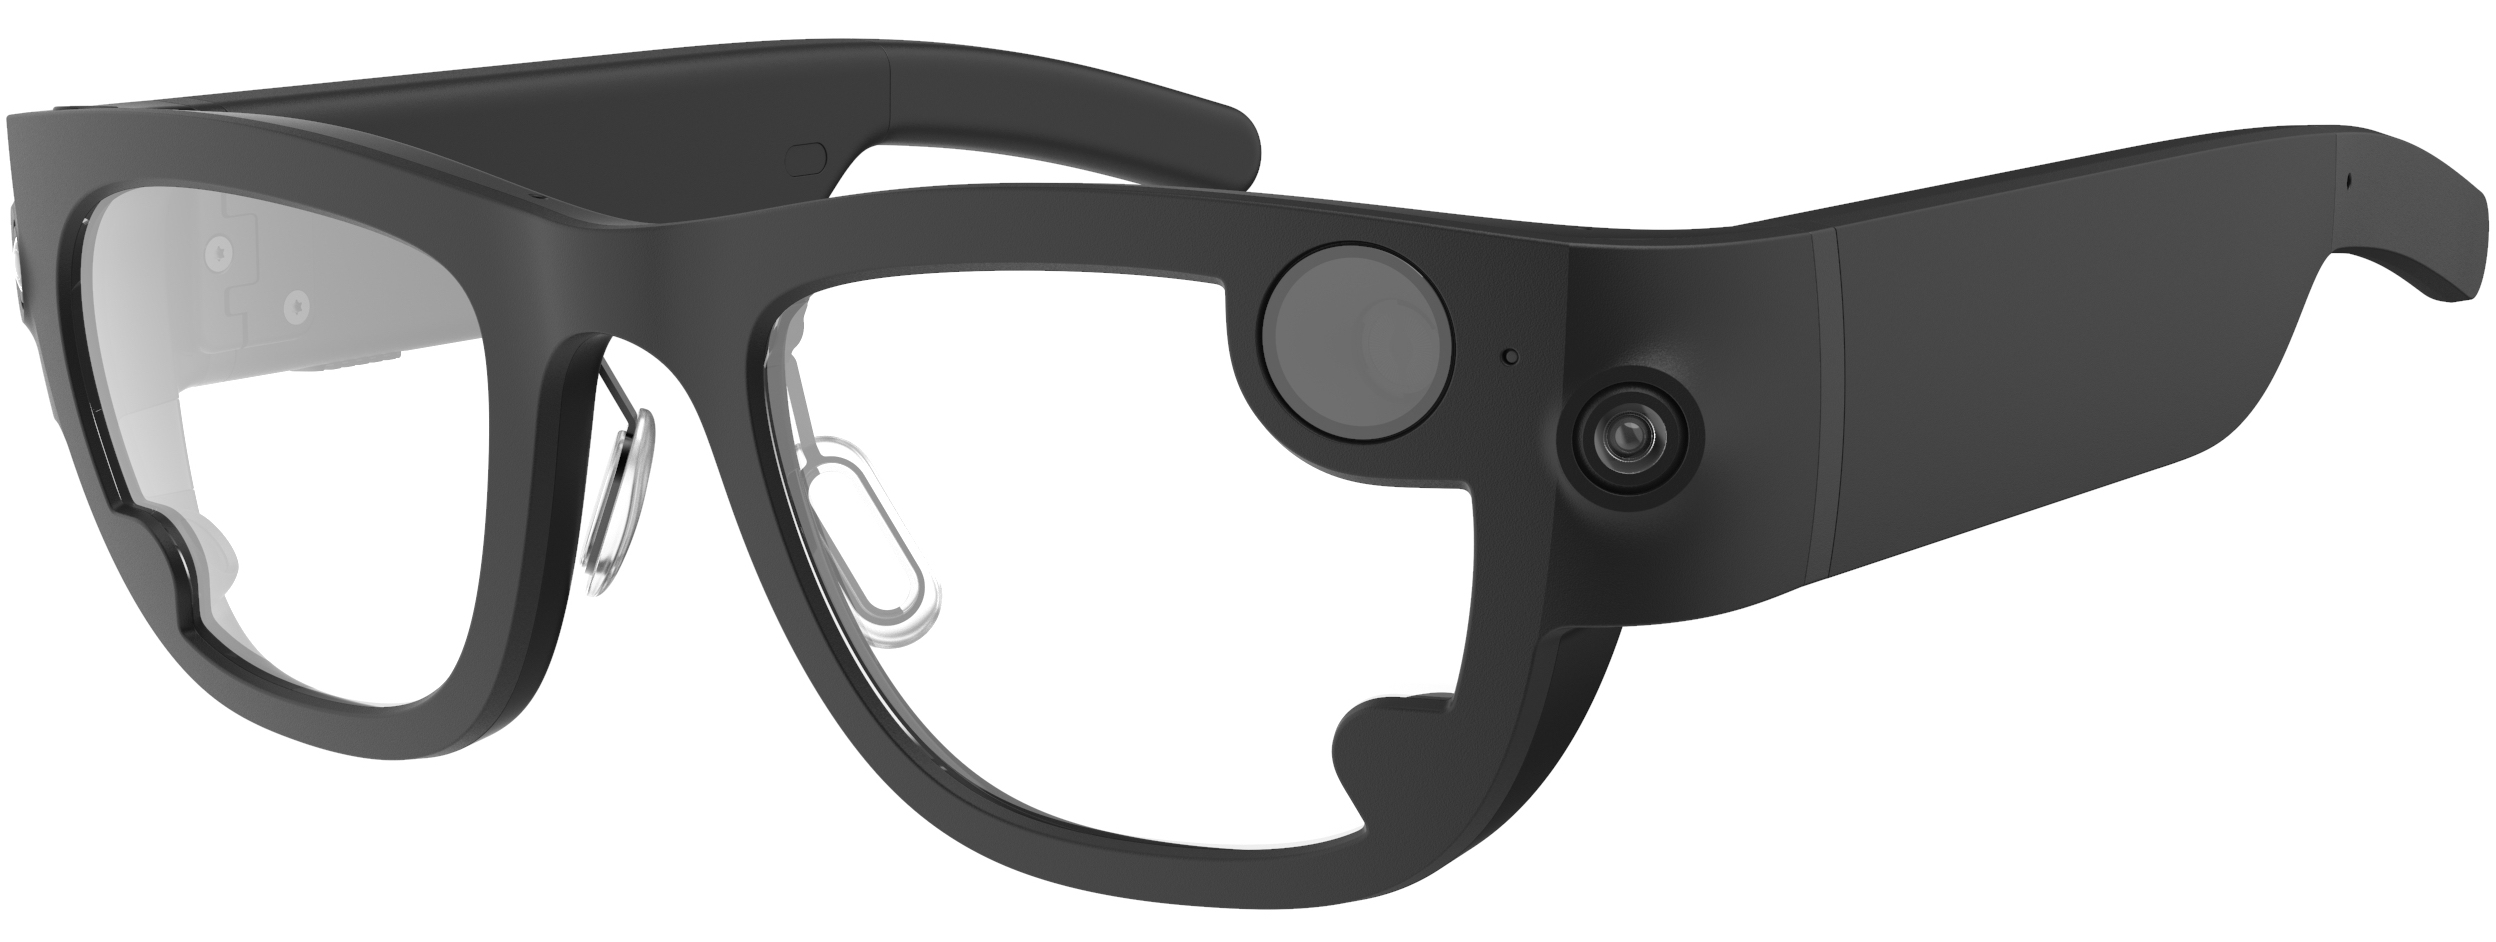
\includegraphics[width=\textwidth]{img/intro/aria.gen1.png}
%        \caption{Aria Gen1.}
        \label{fig:aria_gen1}
    \end{subfigure}
    \hfill
    \begin{subfigure}[b]{0.30\textwidth}
        \centering
        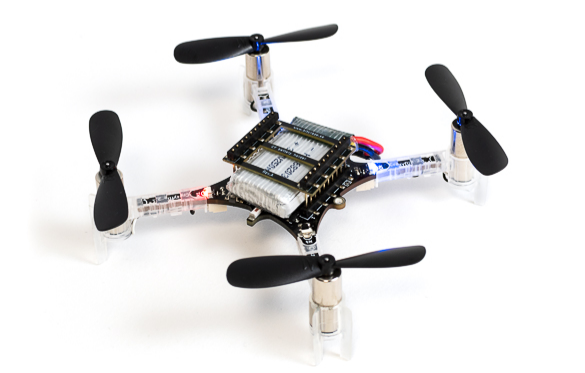
\includegraphics[width=\textwidth]{img/intro/crazyflie.png}
%        \caption{Crazyflie 2.1.}
        \label{fig:crazyflie}
    \end{subfigure}
    \hfill
    \begin{subfigure}[b]{0.30\textwidth}
        \centering
        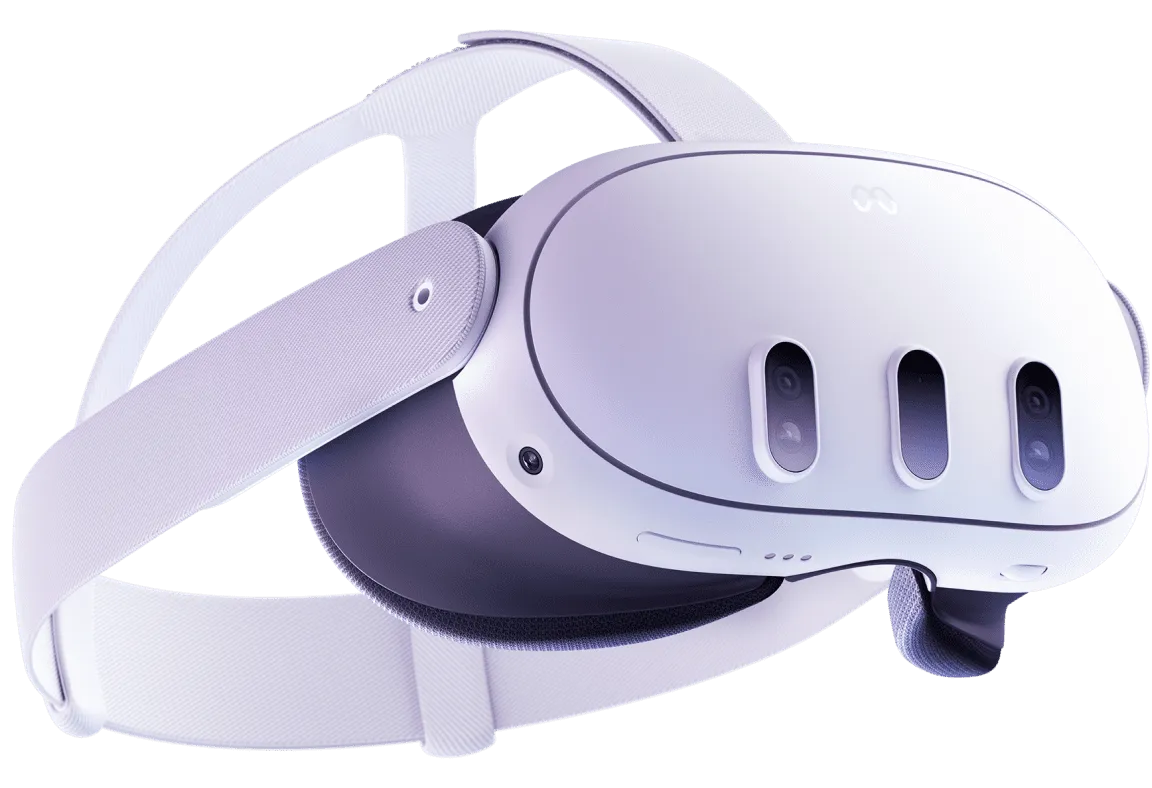
\includegraphics[width=\textwidth]{img/intro/metaquest3.png}
%        \caption{Meta Quest 3.}
        \label{fig:metaquest}
    \end{subfigure}
    \caption{Ejemplos representativos del espectro de plataformas que emplean VI-SLAM: el Project Aria Gen1 (lentes de realidad aumentada de investigación), el Crazyflie~2.1 (nano drone de bajo costo) y el Meta Quest~3 (headset de VR/AR de consumo masivo).}
    \label{fig:devices}
\end{figure}
